% % Second Chapter : Theoritical Approach
%
% Master Thesis: Calibration and fusion of stereo cameras and optical-range finder sensors
% for in-space localization and mapping
%
% Achieved at Space System Lab, M.I.T.
% Supervisor: Alvar Saenz-Otero, Daniel Alazard
%
% Institut Sup�rieur de l'A�ronautique et de l'Espace
% Major: Telecommunications et r�seaux - Syst�mes Spatiaux et Lanceurs
% Gabriel Urbain - October 2014
%%

\chapter{Theoretical Approach}

In this chapter, we will try to give the reader all the theoretical tools to understand the algorithm development carried out in this project. The first section aims at reminding background models and theories but we will assume the reader to have basics in mechanics of the rigid body, optics, image processing, numerical analysis and computer sciences.
Section two focuses on calibration algorithm. It reviews solutions found in the literature to calibrate separately stereoscopic cameras and TOF camera but also describes the implementation and adaptation of a new algorithm proposed in \cite{stereo_tof_fusion_proba} to calibrate the whole TOF and stereo cameras system while taking advantage of each sensors characteristics.
Finally, the last section analyzes the core implementation of the fusion algorithm tested in this project, try to set out arguments to the choices that have been made and describes each parts in details.

\section{Background}
Before going into further details into the algorithms breakdown, it may be necessary to clarify the models employed throughout this document. Indeed, to simplify the sensor fusion analysis and implementation, we will have to make numerous simplifications and hypothesis about the camera models that we shall remember in Chapter 4 where experimental results are discussed.

\subsection{Mathematical Notations}
Several coordinates systems are used in this work leading themselves to many different transformations between each others. To give the reader a better overview, this paragraph summarizes the mathematical notations employed in this document.

\paragraph{Coordinates Systems:}

\paragraph{Transformations Matrices:}

\subsection{Pinhole Camera Model}
According to \cite{epipolar_geometry}, a common representation of a camera is composed of a lens represented by a single pinhole $O$ in the \textit{focal plane }$\mathcal{F}$ and a sensor matrix in the \textit{image plane} $\mathcal{I}$ at a distance $f$ from the focal plane. As represented on figure \ref{fig:cam1}, $O$, also called optical center, is the origin of the world 3D coordinates system $OXYZ$ where $Z$ is perpendicular to the focal plane and directed in the opposite direction of the image plane and $X$ and $Y$ are included in the plane. The pixels on the image plane are localized with a 2D coordinates system $O'U'V'$ where the origin is situated on the lower-right corner of the sensor matrix. The $Z$ axis intersects $\mathcal{I}$ in a point $c' = (c_u', c_v')$ called the \textit{principal point}.

% Figure cam1
\begin{figure}[!htt]
	\begin{center}
		\label{fig:cam1}
		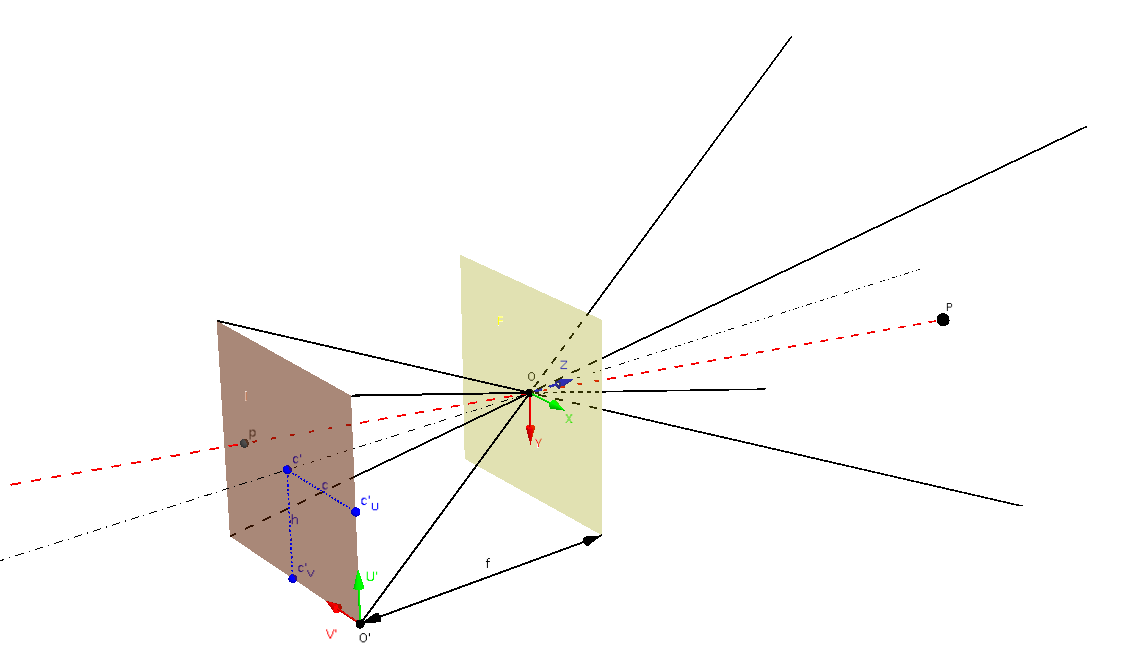
\includegraphics[width=15cm]{img/cam1.png}
		\caption{Geometry of the pinhole model for a single camera}
	\end{center}
\end{figure}

To facilitate the representation, we can consider a \textit{virtual image plane} at a distance $f$ on the positive $Z$ axis, which doesn't change anything to the problem but helps to recreate directly a \textit{projected image} with the same orientation than the real object. We now have a 2D coordinate system $O"UV$ (figure \ref{fig:cam2}).

% Figure cam2
\begin{figure}[!htt]
	\begin{center}
		\label{fig:cam2}
		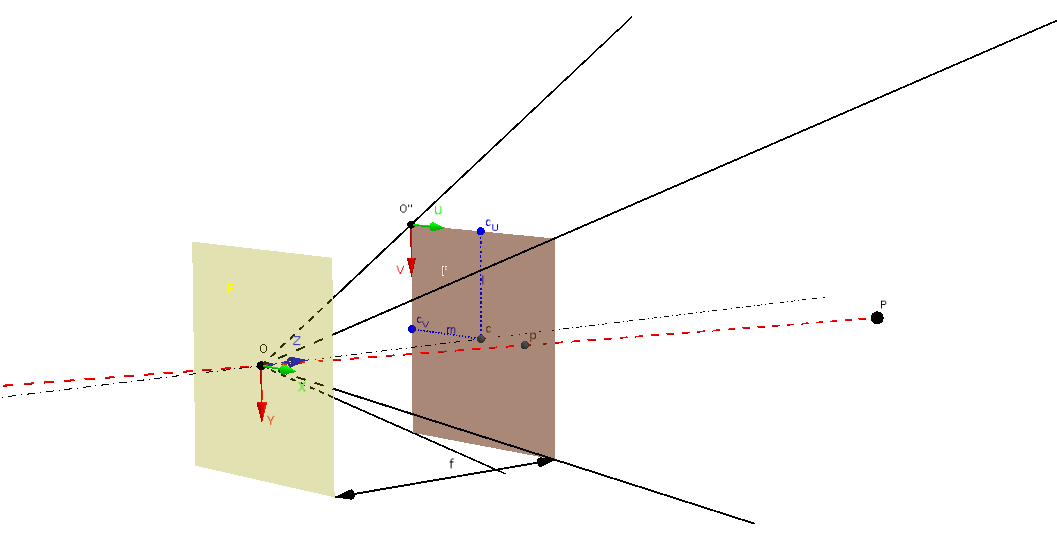
\includegraphics[width=15cm]{img/cam2.png}
		\caption{In this simplified representation, the point P is projected in the virtual plane}
	\end{center}
\end{figure}

In this optimal model, the \textit{intrinsic} geometry of the camera is completely represented by the parameters $f$, $c_x$ and $c_y$ measured in pixels. However, to make the model more realistic, we can introduce extra parameters such as:
\begin{itemize}
\item The lens enlargement $k$, whose value is different along $u$ and $v$ axis and represented in the model by coordinates $f_u = k_u * f$ and $f_v = k_v * f$
\item The skew $s_{uv}$, assessing the non-orthogonality between rows and columns of the sensor photosensitive cells.
\end{itemize}
Those five parameters $f_u$, $f_v$, $c_u$, $c_v$, $s_{uv}$ constitute what we call the \textit{intrinsic matrix} of the camera:
\begin{equation}
K =  \begin{pmatrix}
	f_u & s_{uv} & c_u\\
	0 & f_v & c_v\\
	0 & 0 & 1
	\end{pmatrix}
\end{equation}

Therefore, we can write the affine transformation linking a \textit{world point}, represented by its \textit{homogeneous coordinates} in the camera 3D coordinates system and a \textit{projected point} represented by its \textit{homogeneous coordinates} in the image 2D coordinates system:
\begin{equation}
\label{eq:pinhole}
s \begin{pmatrix}[0.8]
u\\
v\\
1
\end{pmatrix}
 = K * \begin{pmatrix}[0.8]
 x\\
 y\\
 z\\
 1
 	\end{pmatrix}
\end{equation}

Finally, the model can be refine to take the distortions into account. As proposed by Brown \cite{camera_distortion}, the distortion may be divided into radial and tangential and can be represented by a second degree polynomial which map the undistorted and distorted images together thanks to 6 parameters. This will be detailed in section \ref{sec:calib}.\\

One should also notice that the parameters discussed here define the camera mathematical model but performances can be determined as well. For instance, the \textit{Field-Of-View} (FOV) of the camera and the pixel size $\epsilon_p$ of the photosensitive cells (sometimes given by the pixel density, measured in pix/meters) are two characteristics to measure camera performances.

\subsection{Stereoscopic Cameras Model}
In the literature, the stereo camera is commonly represented as the assembly of two pinhole model whose focal points are separated by a distance called \textit{baseline}. As in figure \ref{fig:cam_stereo}, we thus have now two 3D coordinate systems $L = O_LX_LY_LZ_L$ and $R = O_RX_RY_RZ_R$.

% Figure cam_stereo
\begin{figure}[!htt]
	\begin{center}
		\label{fig:cam_stereo}
		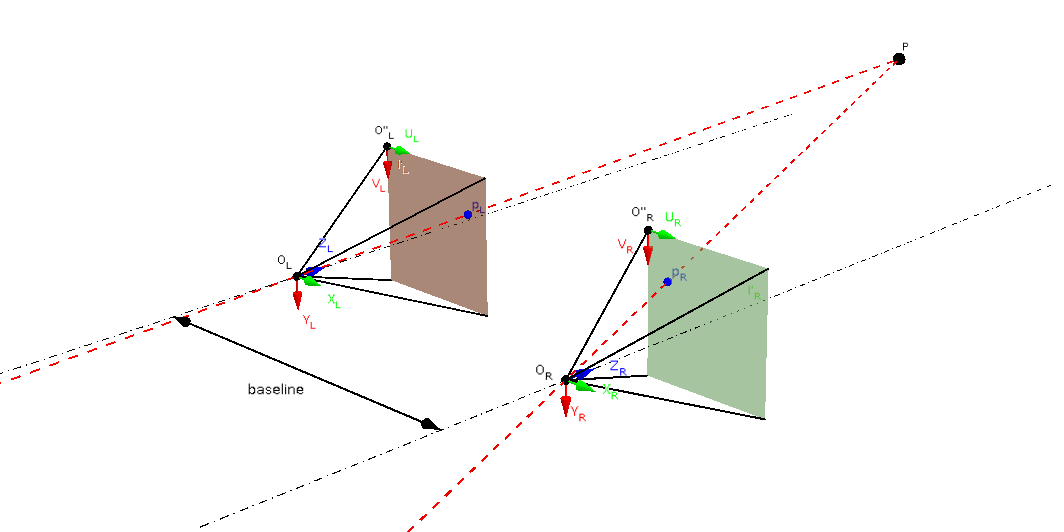
\includegraphics[width=15cm]{img/cam_stereo.png}
		\caption{Model of a stereoscopic cameras assembly}
	\end{center}
\end{figure}

\subsubsection{Projection}
We can still use the model developed in the precedent paragraph the rotation and the translation between $L$ and $R$ must be taken into account when a point is represented in 3D. An \textit{extrincic matrix} is then defined to perform that transformation:
\begin{equation}
M =  \begin{pmatrix}
	r_{X,X'} & r_{X,Y'} & r_{X,Z'} & t_{X}\\
	r_{Y,X'} & r_{Y,Y'} & r_{Y,Z'} & t_{Y}\\
	r_{Z,X'} & r_{Z,Y'} & r_{Z,Z'} & t_{Z}
	\end{pmatrix}
\end{equation}

Which gives:
\begin{equation}
s \begin{pmatrix}
u\\
v\\
1
\end{pmatrix}
 = K * M * \begin{pmatrix}[0.8]
 x\\
 y\\
 z\\
 1
 	\end{pmatrix} = P * \begin{pmatrix}[0.8]
 	 x\\
 	 y\\
 	 z\\
 	 1
 	 	\end{pmatrix}
\end{equation}

Where $P$ is also called the \textit{projection matrix}.

When we write the equations for both left and right cameras, the \textit{extrinsic matrix} can either refer to a third coordinates system, either to $L$ or $R$. In the last case, one of the two $M$ matrix is useless. For instance, if we consider the world coordinates system as $L$, we now write:
\begin{equation}
\label{eq:stereo}
\begin{cases}
s \begin{pmatrix}[0.8]
	u_L\\
	v_L\\
	1
	\end{pmatrix}
= K_L * \begin{pmatrix}[0.8]
	x\\
	y\\
	z\\
	1
	\end{pmatrix}\\
s \begin{pmatrix}[0.8]
	u_R\\
	v_R\\
	1
	\end{pmatrix}
= K_R * M_R * \begin{pmatrix}[0.8]
	x\\
	y\\
	z\\
	1
	\end{pmatrix}
\end{cases}
\end{equation}

As for the camera model, those equations can be used to compute directly the $(u_L, v_L)$ and $(u_R,v_R)$ coordinates from the 3D coordinates of a point with the knowledge of \textit{intrinsic} and \textit{extrinsic} matrices for both cameras. This process is known as \textit{\textbf{projection}}.

\subsubsection{Triangulation}
Intuitively, if inverting the pinhole equation was not directly useful with a mono camera because there was one degree of freedom remaining, we can invert the stereo cameras model to find the 3D coordinates from the projected points in $L$ and $R$. This process, known as \textit{\textbf{triangulation}}, however requires the triangulated points to respect the \textit{epipolar constraint} to give coherent results \cite{multiple_view}, \textbf{i.e.} $(u_L,v_L)$ and $(u_R, v_R)$ must be defined such as the two \textit{epipolar rays} from $L$ and $R$ cross in one point in the real world as represented infigure \ref{fig:cam_stereo}.

Practically, in the 3D reconstruction from stereo sensors problem, the points $p_L = (u_L, v_L)$ and $p_R = (u_R, v_R)$ in the focal images are found using image processing techniques, as developed in \ref{subsec:fusion:overview}. The precision of this method, the accuracy of the physical sensors, the precision of the calibration matrices, the numerical errors,... Everything make this constraint difficult to respect. We can therefore consider two ways to overcome this issue:
\paragraph{Simplify the problem}: In the first option, we suppose the cameras to be perfectly aligned in $Y$ and $Z$ coordinates, the \textit{baseline} is measured on the $X$ axis. Thus, \textit{epipolar lines} are totally included in $XZ$ planes for each points and as soon as those one are visible in left and right images, they will cross for sure. This leads to simplified projection matrices:
\begin{equation}
P_L = \begin{pmatrix}
	f_u & 0 & c_u & 0\\
	0 & f_v & c_v & 0\\
	0 & 0 & 0 & 0
	\end{pmatrix}
\end{equation}
\begin{equation}
P_R = \begin{pmatrix}
	f_u & 0 & c_u & T_R\\
	0 & f_v & c_v & 0\\
	0 & 0 & 0 & 0
	\end{pmatrix}
\end{equation}

\paragraph{Minimize errors}: The other solution is to keep an elaborate model where left and right cameras can be misaligned but try to minimize the sum of euclidean errors when we are triangulating many points. Various algorithm concerning the subject have been analyzed in \cite{multiple_view} or \cite{triangulation}.

The two kinds of \textit{triangulation} and \textit{projection} methods have been implemented in the stereo cameras software but this thesis mostly focus on the first one for it is easier to implement and give sufficient results with VERTIGO \cite{muggler_phd}.

\subsection{Optical Range Finder Model}
According to \cite{TOF_principle} and \cite{SR4k_manual}

\section{Calibration Algorithm}
\label{sec:calib}
\subsection{Optical Range Finder Calibration}
\subsection{Overview}
\subsection{Architecture}
\subsection{Stereoscopic Cameras Calibration}
\subsection{Overview}
\subsection{Architecture}
\subsection{Multi-Sensors Calibration}
\subsection{Overview}
\subsection{Architecture}
\subsection{Checkerboard Points Detection}
\subsection{Stereoscopic Triangulation}
\subsection{Optical Range Finder Pinhole Inversion}
\subsection{Pose Estimation}

\section{Fusion Algorithm}
\subsection{Overview}
\label{subsec:fusion:overview}
\subsection{Architecture}
\subsection{Determination of the Points Framed by all Cameras}
\subsection{Optical Range Finder Noise Model}
\subsection{Probabilistic Space Discretization}
\subsection{Optical Range Finder Probabilistic Model}
\subsection{Stereoscopic Cameras Model}
\subsection{Joint Probability Computation}
\subsection{Depth Estimation Selection}
\subsection{3D Coordinates Computation}
\subsection{Point Cloud Creation}